% !TEX root = ../main.tex
\documentclass[../main.tex]{subfiles}
\begin{document}
\section{Анализ предметной области}

В настоящий момент на рынке есть много решений в области цифровых стетоскопов. Приведем несколько примеров и проанализируем плюсы и минусы.

\subsection{3M™ Littmann® Electronic Stethoscope Model 3200}
\begin{figure}[H]
\centering
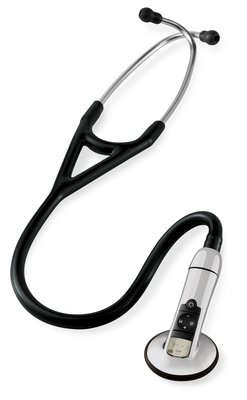
\includegraphics[width=6cm]{images/littmann.jpg}
\caption{3M™ Littmann® Electronic Stethoscope Model 3200}
\end{figure}

Технические характеристики стетоскопа представленного на рисунке 1:
\begin{itemize}
  \item Диапазон принимаемого сигнала: 10 - 2000Гц
  \item Возможность записи 12ти 30-секундных звуковых дорожек
  \item Передача данных через Bluetooth
  \item Удаленная прослушка с помощью технологии 3M™ Littmann® TeleSteth™
  \item Удаление 85\% (в среднем) окружающего шума
  \item 24х кратное усиление сигнала
  \item Цена - 22000 руб
  \item Вес - 185г
\end{itemize}

Полное описание стетоскопа можно увидеть по ссылке \cite{littmann}

Это один из самых лучших стетоскопов, существующих на рынке. Стетоскоп обеспечивает высокое качества звука, но только в нижнем диапазоне (до 2кГц). Также к плюсам нужно отнести высокое качество подавления окружающего шума. Минусом является высокая цена.

\subsection{CMS-VESD SPO2 PR}
\begin{figure}[H]
\centering
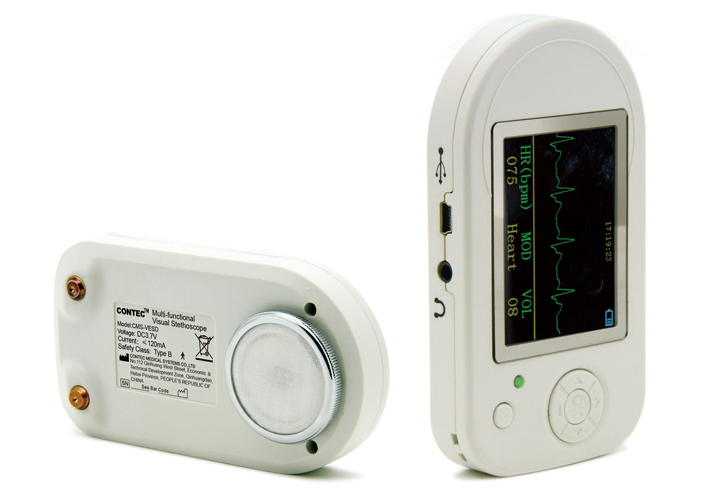
\includegraphics[width=11cm]{images/cms-vesd.jpg}
\caption{CMS-VESD SPO2 PR}
\end{figure}

Технические характеристики  стетоскопа представленного на рисунке 2:
\begin{itemize}
  \item Диапазон принимаемого сигнала для сердца: 20 - 230Гц
  \item Диапазон принимаемого сигнала для легких: 100 - 800Гц
  \item Диапазон принимаемого сигнала для сердца и легких: 20 - 800Гц
  \item Измерение пульса: 30 - 300 ударов в минуту
  \item Точность измерения пульса: +- 2 уд/мин
  \item Диапазон измерения насыщения кислородом (SpO2, процентное содержание оксигемоглобина в артериальной крови): 70\% - 100\%
  \item Дисплей, отображающий в реальном времени звуковую волну, пульс, SpO2
  \item Возможность загрузки данных на компьютер через USB
  \item ПО для анализа данных
  \item Цена - 5800руб
  \item Вес - 100г
\end{itemize}

Полное описание стетоскопа можно увидеть по ссылке \cite{cms-vesd}

Данный стетоскоп обладает невысокой разрешаюшей способностью (маленький диапазон принимаемого сигнала для сердца и легких) и невысокой ценой.

\subsection{CMS-VE}
\begin{figure}[H]
\centering
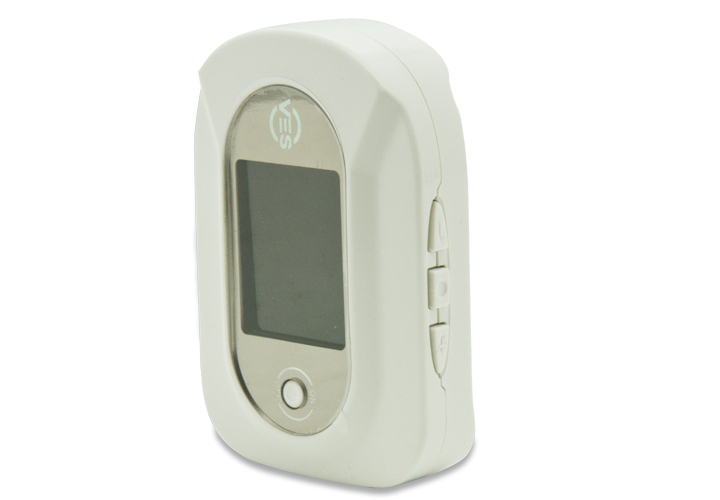
\includegraphics[width=11cm]{images/cms-ve}
\caption{CMS-VE}
\end{figure}

Технические характеристики стетоскопа представленного на рисунке 3:
\begin{itemize}
  \item Диапазон принимаемого сигнала для сердца: 20 - 230Гц
  \item Диапазон принимаемого сигнала для легких: 100 - 800Гц
  \item Диапазон принимаемого сигнала для сердца и легких: 20 - 800Гц
  \item Измерение пульса: 30 - 300 ударов в минуту
  \item Точность измерения пульса: +- 2 уд/мин
  \item Диапазон измерения насыщения кислородом (SpO2, процентное содержание оксигемоглобина в артериальной крови): 70\% - 100\%
  \item Дисплей, отображающий в реальном времени звуковую волну, пульс, SpO2
  \item возможность загрузки данных на компьютер через USB
  \item ПО для анализа данных
  \item Цена - 5646руб
  \item вес - 100г
\end{itemize}

Полное описание стетоскопа можно увидеть по ссылке \cite{cms-ve}

Преимуществом данного прибора является возможность записывать процентное содержание оксигемоглобина в артериальной крови (SpO2). Недостатками являются невысокая разрешающая способность 20 - 800Гц

\subsection{CMS-M}
\begin{figure}[H]
\centering
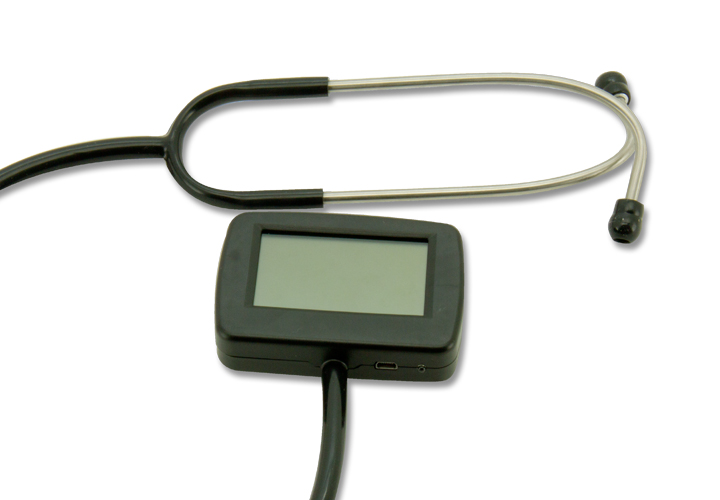
\includegraphics[width=11cm]{images/cms-m}
\caption{CMS-M}
\end{figure}

Технические характеристики стетоскопа представленного на рисунке 4:
\begin{itemize}
  \item Измерение пульса: 30 - 300 ударов в минуту
  \item Точность измерения пульса: +- 2 уд/мин
  \item Диапазон измерения насыщения кислородом (SpO2, процентное содержание оксигемоглобина в артериальной крови): 70\% - 100\%
  \item Дисплей, отображающий в реальном времени звуковую волну, пульс, SpO2
  \item возможность загрузки данных на компьютер через USB
  \item ПО для анализа данных
  \item Цена - 6500руб
\end{itemize}

Полное описание стетоскопа можно увидеть по ссылке \cite{cms-m}

Преимуществом данного прибора является возможность записывать процентное содержание оксигемоглобина в артериальной крови. ) Недостатком является невысокая разрешающая способность 20 - 800Гц

\subsection{Cardionics E-scope II}
\begin{figure}[H]
\centering
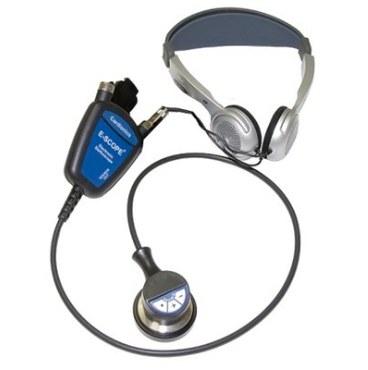
\includegraphics[width=11cm]{images/e-scope}
\caption{Cardionics E-scope II}
\end{figure}

Технические характеристики стетоскопа представленного на рисунке 5:
\begin{itemize}
  \item Диапазон 45-900Hz для звуков сердца и 50-2000Hz
  \item 30-ти кратное усиление сигнала по сравнению с акустическим стетоскопом.
  \item вход для наушников
  \item возможность подключиться к компьютеру через USB-кабель для визуализации сигнала
  \item переключатель между звуками сердци и звуками легких
  \item Цена - 20900руб
\end{itemize}

Полное описание стетоскопа можно увидеть по ссылке \cite{cardioics}

Преимуществами данного прибора являеются достаточно высокий, по сравнению с другими аналогами, диапазн принимаемого сигнала (20 - 2000Гц) и возможность подключится к к компьютеру для визуализации сигнала) Недостатком является высокая цена.

\subsection{Thinklabs One}
\begin{figure}[H]
\centering
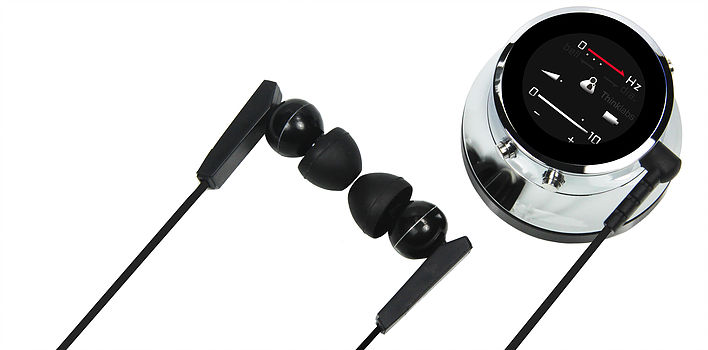
\includegraphics[width=11cm]{images/thinklabs-one}
\caption{Thinklabs One}
\end{figure}

Технические характеристики стетоскопа представленного на рисунке 6:
\begin{itemize}
  \item диапазон 10-1000Гц
  \item более чем 100 кратное усиление сигнала по сравнению с акустическим стетоскопом.
  \item система аудио-фильтров: несколько фильтров дают возможность контроллировать множество нюансов выходного сигнала
  \item шумоподавление
  \item возможность подключиться к iPhone, iPad, Android, планшету, компьютеру.
  \item управление устройством и запись сигнала через мобильное приложение
\end{itemize}

Полное описание стетоскопа можно увидеть по ссылке \cite{thinklabs-one}

Преимуществом данного прибора является наличие качественных приложений под основные операционные системы (iPhone, iPad, Android, macOS, Windiws) Недостатком является то что приложения с закрытым исходным кодом, что делает невозможным модификацию програмного обеспечения под свои нужды.

\subsection{Eko Core}
\begin{figure}[H]
\centering
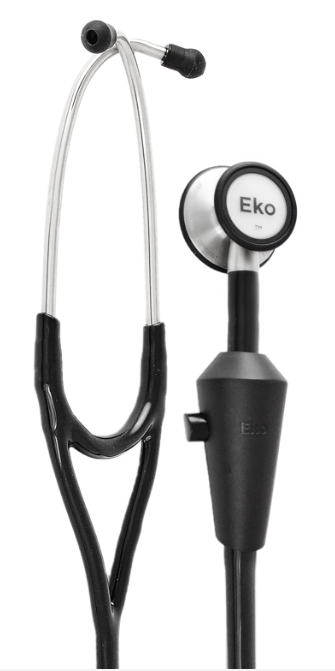
\includegraphics[width=7cm]{images/eko-core}
\caption{Eko Core}
\end{figure}

Технические характеристики  стетоскопа представленного на рисунке 7:
\begin{itemize}
  \item 40-кратное усиление сигнала
  \item Частота дискретезации 4000Гц
  \item Диапазон 20Гц – 2kГц
  \item Запись в .WAV формат
  \item Подключение через Bluetooth 4.0 low-energy
  \item Програмное обеспечение для iOS, Android, Windows
\end{itemize}

Полное описание стетоскопа можно увидеть по ссылке \cite{eko-core}

Преимуществом данного прибора является беспроводная передача данных через Bluetooth и наличие приложений под основные операционные системы (iPhone, iPad, Android, macOS, Windiws). Недостатком является то что приложения с закрытым исходным кодом, что делает невозможным модификацию програмного обеспечения под свои нужды.

\subsection{Eko Duo}
\begin{figure}[H]
\centering
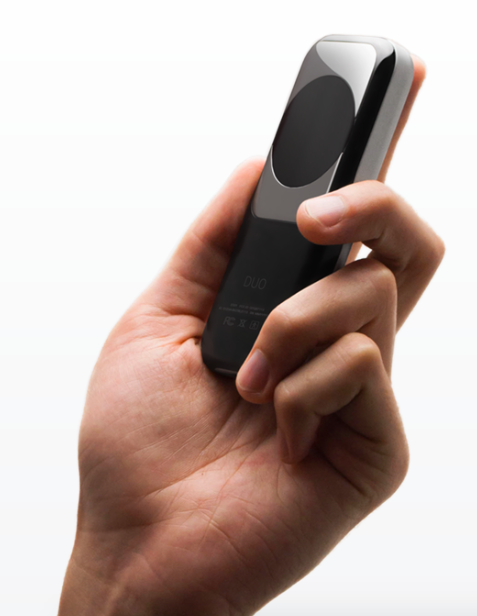
\includegraphics[width=7cm]{images/eko-duo}
\caption{Eko Core}
\end{figure}

Технические характеристики \cite{eko-duo} стетоскопа представленного на рисунке 8:
\begin{itemize}
  \item 60-кратное усиление сигнала
  \item подавление окружающего шума
  \item Частота дискретезации 4000Гц
  \item Диапазон 20Гц – 2kГц
  \item 4 аудиофильтра
  \item Запись в .WAV формат
  \item Подключение через Bluetooth 4.0 low-energy
  \item Програмное обеспечение для iOS, Android, Windows
  \item Возможность снимать ЭКГ
\end{itemize}

Полное описание стетоскопа можно увидеть по ссылке \cite{eko-duo}

Преимуществом данного прибора является относительно высокая частота дискретизации (4000Гц), наличие аудиофильтров и качественное шумоподавление. Недостатком является програмное обеспечение с закрытым исходным кодом без возможности модифицировать его для своих задач.
% \subsection{EM410}
% Диапазон принимаемого сигнала: 100Гц - 10кГц, цена 3500руб.\\

Как видно из списка товаров, большинство стетоскопов не имеют возможность анализировать сигнал выше 1000 Гц. Те же которые имеют - дорого стоят. Многие дешевые стетоскопы вообще нацелены на измерение пульса, а не на подробный анализ звука.
\newpage

\end{document}
